\documentclass[conference]{IEEEtran}
\usepackage{times}

% numbers option provides compact numerical references in the text. 
\usepackage[numbers]{natbib}
\usepackage{soul,xcolor,amsmath, amssymb, fbox, graphicx, pdfpages, breqn}
\usepackage[bookmarks=true]{hyperref}
\usepackage{parskip, graphicx}

\pdfinfo{
   /Author (Martin Braquet and Steven Patrick)
   /Title  (Robot Learning Project Milestone)
   /Subject (Robots)
}

\begin{document}

% paper title
\title{CS391R - Robot Learning: Final Report\\ \large \textit{Reinforcement Learning for Cooperative Manipulation}}

% You will get a Paper-ID when submitting a pdf file to the conference system
\author{\IEEEauthorblockN{Martin Braquet}
\and
\IEEEauthorblockN{Steven Patrick}}

\maketitle

\thispagestyle{plain}
\pagestyle{plain}

\begin{abstract}
This project aims at building a reinforcement learning algorithm where multiple agents cooperatively move an object. Our solution to accomplish this task we defined an intrinsic reward based on the work from \cite{DBLB}. We improved upon their original design by changing the training method from Proximal Policy Optimization (PPO) to Deep Deterministic Policy Gradient (DDPG). We also added a hindsight experience replay (HER) buffer to the training phase. This resulted in a faster convergence to a successful policy than the previous approach. We demonstrated our approach in multiple manipulation tasks such as OpenAI's Fetch pick-and-place task and Robosuite's two arm lifting task.
\end{abstract}

\IEEEpeerreviewmaketitle

\section{Introduction}\label{sec:introduction}

The field of robotic manipulation has become an important challenge due to its wide applicability to real-world problems. Fulfilment centers often have human workers preparing packages for delivery which can be a tedious task prone to mistakes. Robot's have largely not been involved in the process due to the complexities involved with manipulating novel objects in cluttered environments. Another problem that is waiting to be solved is manipulating larger objects. User's could buy a large robot that is capable of moving heavy objects, but it is typically more cost effective to buy multiple smaller robots to accomplish the task collectively. Applications in the real-world for this problem include moving furniture around the house, moving bins around a factory, and using heavy machinery that requires a high degree of maneuverability.

This latter problem of moving large obstacles is the motivation for our project. In this paper, we present an improvement on a multi-agent reinforcement learning architecture. The original work \cite{DBLB} combines extrinsic reward defined by completing a task with an intrinsic reward that rewards collective actions over individual ones. This prevents the various agents from acting greedily and not being able to complete a task. The learned policy is a global policy and is found through an actor-critic scheme. They were able to demonstrate their approach on multiple different tasks including multi-agent manipulation. 

Our improvement is turning their proposed on-policy approach to Deep Deterministic Policy Gradient (DDPG) with Hindsight Experience Replay (HER) in order to better use the data generated by interacting with the environment. We propose that our method explores the solution space more effectively and converges to a solution faster that the original work. We demonstrate our approach on multiple environments involving robotic arms manipulating a desired object. Our source code is available at \url{https://github.com/spatric5/robosuite}.

In order to solve this problem, we started the implementation of a simple single-agent reinforcement learning algorithm, DDPG, where one robotic arm is required to pick a hammer on a table (see Fig. \ref{environment_onerobot}).

\begin{figure}[h!]
    \centering
    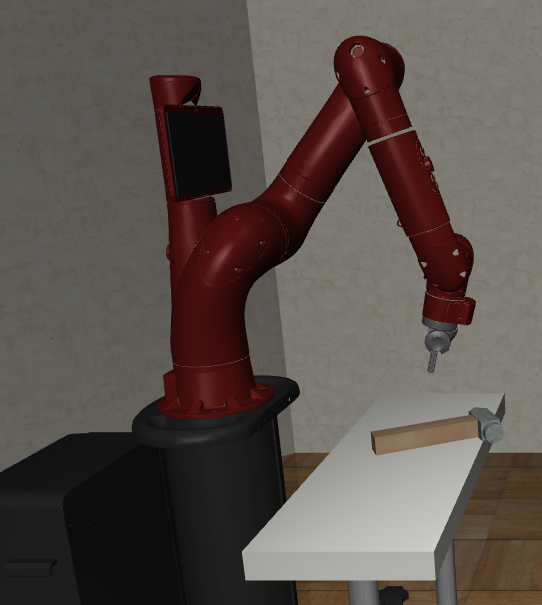
\includegraphics[width=0.35\textwidth]{EnviOneRobot.png}
    \caption{Environment with only one robot which aims at picking the hammer}
    \label{environment_onerobot}
\end{figure}

Next, we extend the work to two agents using the algorithm in \cite{DBLB}, which are described in Section \ref{techApp}. We obtain a high success using the DDPG and DDPG-HER algorithms in multiple manipulation tasks such as OpenAI's Fetch pick-and-place task and Robosuite's two arm lifting task.

The following of the paper is organized as follows. Section \ref{sec:prob} provides a definition of the problem. Section \ref{sec:related_work} presents a literature review of the work related to our problem. Section \ref{sec:data} shows the data and simulation environments used for this project. Section \ref{techApp} presents the technical detail of our approach, specifically the architecture of the neural network. Finally, Section \ref{sec:simu} analyses the simulation results and Section \ref{sec:ccl} concludes this final report.

\section{Problem statement} \label{sec:prob}

Our demonstration case is two agents carrying a large object through a static environment with multiple obstacles. These obstacles force the robots to maintain their grip on an object while executing changes in team formation or object orientation.

No specific dataset is used, instead we use online training by making the agents explore and then exploit the set of actions allowing them to reach the goal. We expect the two robots to carry an object (for example a hammer or a heavy bar). The objective is considered to be fulfilled once the object is lifted by the two robots and is not in contact with the table anymore.

The results are evaluated compared to the random policy (and the benchmark SAC policy available on the Robosuite website if available). More precisely, we analyze the success rate in function of the number of iteration steps for the respective algorithms. Our algorithm performs significantly better than the random policy algorithm, reaching a success rate above 90\%.

\section{Related Work}\label{sec:related_work}

\subsection{Single-Agent Reinforcement Learning}

The single agent reinforcement learning framework is based on the model of Figure \ref{SARL}, where an agent interacts with the environment by selecting actions to take and then perceiving the effects of those actions, a new state and a reward signal indicating if it has reached some goal.

\begin{figure}[h!]
    \centering
    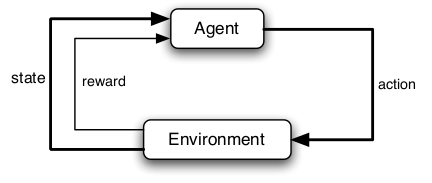
\includegraphics[width=0.45\textwidth]{SARL.png}
    \caption{General reinforcement learning task.}
    \label{SARL}
\end{figure}

The objective of the agent is to maximize some measure over the rewards, such as the sum of all rewards after a number of actions taken. This general idea can be described by the framework of Markov decision processes \cite{bellman1957}, over which the solutions for the reinforcement learning problem are constructed \cite{Sutton1998}.

They can be defined as a tuple
$(S, A, T, R)$ where $A$ is an action set, $S$ is a state space, $T$ is a transition function defined as a probability distribution over the states, and $R$ is a reward function representing the expected value of the next reward.

\begin{figure*}[htbp]
    \centering
    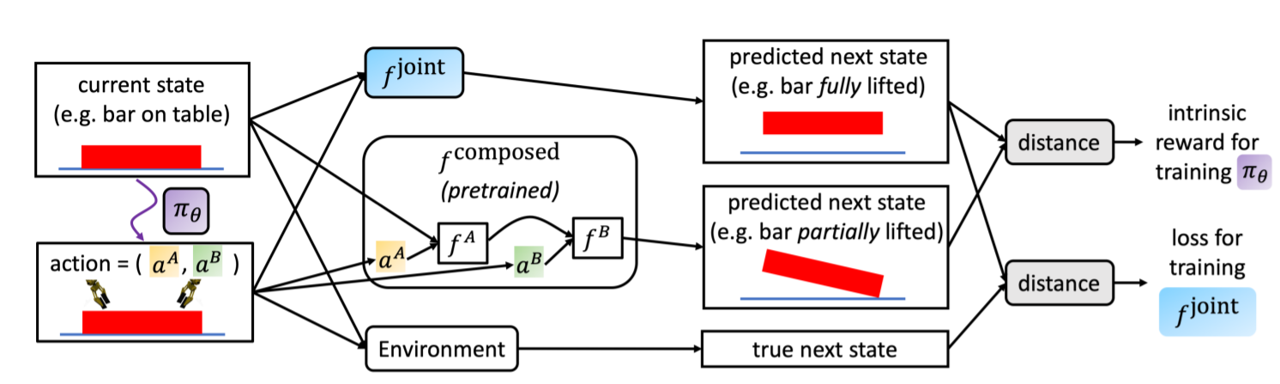
\includegraphics[width=\textwidth]{Architecture.png}
    \caption{Overview of network architecture. This figure is pulled from \cite{DBLB}}
    \label{Network_Arch}
\end{figure*}

\subsection{Multi-Agent Reinforcement Learning}

Multi-agent systems are rapidly finding applications in a wide variety of domains such as robotic teams \cite{dudek1996taxonomy}, distributed control \cite{yu2013distributed}, collaborative decision support systems (e.g., stock trading \cite{luo2002multi}), human-robot interactions \cite{laengle2001human}, data mining \cite{Cao2009}, etc.

Less research has been done for the control of multi-agent systems compared to the single-agent case (especially in reinforcement learning). Nonetheless the multi-agent setting can be clearly formulated as a Markov game instead of a Markov decision process as in the single-agent case \cite{littman1994markov}. More precisely, they can be defined as a tuple $(S, A, T, R)$ where $A$ is a joint action set, $S$ is a joint state space, $T$ is a transition function defined as a probability distribution over the states, and $R$ is a reward function representing the expected value of the next reward. Note that the state transitions and the agent rewards depend on the joint action. The Q-function of each agent also depends on the joint action and is conditioned on the joint policy


Additionally, the value function does not only depend on the individual policy of each agent but also on the policies of other agents. 
One major problem resides in the presence of multiple agents that interact within a shared environment and learn simultaneously. Due to the co-adaption, the environment dynamics appear \textit{non-stationary} from the perspective of a single agent \cite{bucsoniu2010multi}.

We focus our work on robotic manipulation, which refers to the ways robots interact with the objects around them: grasping an object, opening a door, packing an order into a box, etc. All these actions require robots to plan and control the motion of their hands and arms in an intelligent way. Multi-robot manipulation has been used since they can take the advantage of increased driving power and more flexible configuration to solve difficult problems. These problems require more coordination between the robots, they can for example be handled using a potential field based approach \cite{song2002potential} or an impedance based approach for dual-arm manipulation \cite{erhart2013impedance}.

In the case of cooperative multi-robot object manipulation, using reinforcement learning is a strong tool to obtain a robust solutions in high-dimensional spaces \cite{ding2020distributed}. These have been multiple distributed multi-agent RL approaches designed accordingly. A first one is distributed approximate RL (DA-RL), where each agent applies Q-learning with individual reward functions. A second one is game-theoretic RL (GT-RL), where the agents update their Q-values based on the Nash equilibrium of a bimatrix Q-value game. Other algorithms have focused on object transportation using decentralized deep reinforcement learning where the robots are able to learn abstract features of the task to achieve cooperative behaviors \cite{zhang2020multirobot}. Additionally, some research has been done for multi-robot manipulation where the robots collaborate and provide appropriate feedback to a human \cite{sieber2015multi}. 
Finally, some researchers also designed a framework and software architecture for the deployment of multiple autonomous robots in an unstructured and unknown environment \cite{fierro2002framework}, which allows for a modular and hierarchical approach to programming deliberative and reactive behaviors in autonomous operation.

\subsection{Intrinsic Motivation}

For the purposes of this paper, the extrinsic reward in an environment is the reward gained from accomplishing the goal. In a reach position task, this would be the negative of the distance from the goal position. The intrinsic reward is the reward given to the agent for actions not directly related to the task. In multi-agent systems, this could be the reward for acting in a synergistic way with other agents rather than competitively or independently. Defining this intrinsic reward is what the researchers of \cite{DBLB} attempted. In their paper, they define the intrinsic reward as being the difference in the environment if a single agent acted on an object versus a collective of agents acting in the environment. As an example, Figure \ref{Network_Arch} shows how one agent would lift the bar only partially, but two agents would lift it fully. The bar being lifted would have its extrinsic reward and the difference in height and orientation of the bar from the two environments would be the intrinsic reward. The formal definition of the intrinsic reward as defined by \cite{DBLB} is 
\begin{equation}
    r^{intrinsic}=\|f^{joint}(s,a)-f^{composed}(s,a)\|.
\end{equation}
In the equation $f^{joint}$ and $f^{composed}$ are neural networks whose goal are to estimate the next state of the environment. $f^{joint}$ is trained online with episode data, and $f^{composed}$ is a sequential chaining of pre-trained networks that were trained on single agent environments. This reward can be used to get a gradient to train the network in an actor-critic scheme. The author's of the original worked use proximal-policy optimization (PPO). The creators of Intrinsic motivation were able to show the effectiveness of their approach over several tasks including locomotion, manipulation, and games. In this paper we propose using a different optimization strategy to improve upon their work. Our improvements will be discussed in the subsequent sections.

\subsection{Deep Deterministic Policy Gradient}
To improve upon \cite{DBLB}'s work, we implemented Deep Deterministic Policy Gradient \cite{lillicrap2015continuous}. This training method is an online off-policy method. It is online because it uses data directly generated from trying to execute a given task. It is off-policy because the episodes are generated by following the actor's policy but with injected noise. The benefit of the off-policy method as opposed to on-policy like PPO is the episode data can be reused. For our purposes, generating data is somewhat expensive and being able to reuse the data is extremely useful. The update rule from \cite{lillicrap2015continuous} during training is denoted below.

\begin{gather}
    \nabla_{\theta^\mu}J=\frac{1}{N}\sum_{i}\nabla_a Q(s,a|\theta^Q)|_{s=s_i,a=\mu(s_i)} \nabla_{\theta^\mu}\mu(s|\theta^\mu)|_{s_i} \\
    \theta^{Q'} \leftarrow \tau \theta^Q+(1-\tau)\theta^{Q'}\\
    \theta^{\mu'} \leftarrow \tau \theta^{\mu}+(1-\tau)\theta^{\mu'}
\end{gather}
In the above equation $(s,a)$ are state action pairs, $Q(s,a|\theta^Q)$ is the critic network parameterized by $\theta$, $\mu(s|\theta^{\mu})$ is the actor network parameterized by $\theta$, and $\tau$ is a weighting parameter. The apostrophes denote the parameters of the original network are injected with noise to produce a different network.

\subsection{Hindsight Experience Replay}

Since we used an off-policy method and can reuse acquired episode data, we can add Hindsight Experience Replay \cite{andrychowicz2017hindsight} to our training method. This method involves storing state transitions and using random samplings of them to update the network rather than a single episode from start to finish. When storing the we can augment the state transition database with different goals to determine the reward in the transition. To do this, the reward structure of the goals must be agnostic to previous states which is a core property of Markov Decision Processes. As an example, in pick-and-place operations, minimizing the x, y, and z distances to a goal can be learned independently rather than being tightly coupled in other approaches. Over the coarse of many epochs which consist of a set amount of episode runs, the policy explores the state space of the problem much more effectively due to episode data being collected agnostic to the goal. The author's also claim and demonstrate that this approach also does better with sparse rewards which is a more desirable method of reward shaping. Sparse rewards reflect the user's intention better and are less likely to be exploited by a learned policy \cite{andrychowicz2017hindsight}.

\section{Data}\label{sec:data}

For our experiment, the primary source of data are the observations the robot's produce while executing a policy injected with noise. The training is done online and stored in a database for future hindsight experience replay buffers. 
\subsection{Fetch Environment}
The Fetch simulation environment consists of a stationary robot arm that has 6DOF and an additional degree of freedom for opening and closing a gripper. We used two different tasks: reach and pick-and-place. The objective of the reach task was for the end effector of the robot to reach a desired xyz position with orientation being ignored. For the pick-and-place task, the objective was to move a block from one spot to another. The block did not change in size, orientation, or color between simulations, but the initial position and goal position of the block did change with each simulation. A visual of the reach environment can be seen in Figure \ref{fetch-reach} and the pick-and-place environment in Figure \ref{fetch-pick-place}The observation space is the end effector position, velocity, and opened/closed, the desired object's center of mass and velocity, and the goal position the object is sent to. The action space of this environment is declaring the offset of the current position of gripper and opening or closing the gripper.  For the simple pick-and-place task, we simulated on the order of 50,000 simulation runs with each run lasting 150 time steps. 

\begin{figure}[h]
    \centering
    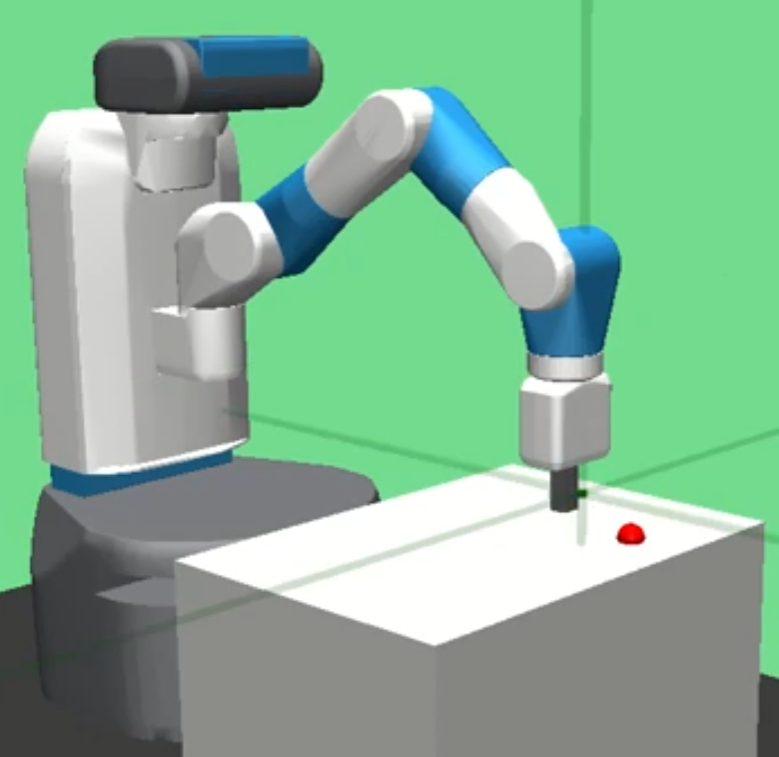
\includegraphics[width=0.4\textwidth]{fetch_reach.png}
    \caption{Fetch Reach environment in Gym Open AI}
    \label{fetch-reach}
\end{figure}

\begin{figure}[h]
    \centering
    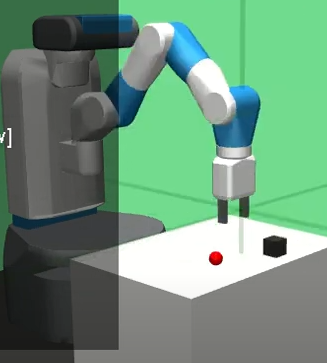
\includegraphics[width=0.3\textwidth]{fetch_pick.png}
    \caption{Fetch pick-and-place environment in Gym Open AI}
    \label{fetch-pick-place}
\end{figure}

\subsection{Robosuite Environment}
The Robosuite environment we used was a single arm lift and a two arm lift. This consisted of one and two 6DOF arms respectively with an extra degree of freedom for each arm of their gripper's being opened or closed. The objective was to move a block in the single arm environment and a bucket in the two arm case to a desired location. The bucket and block did not change in size or color between simulations, but the initial position, orientation, and goal position of the objects did change with each simulation. The visuals for these environments can be seen in Figure \ref{single_arm_env} for the single arm case and Figure \ref{double_arm_env} for the two arm case. The observation space is the end effector position, velocity, and opened/closed and the desired object's center of mass. The action space is similar to the Fetch environment, but the controller could also change the orientation of the end effector. The Robosuite experiment took more runs on the order of 100,000 with the same length of time steps per run.

\begin{figure}[h]
    \centering
    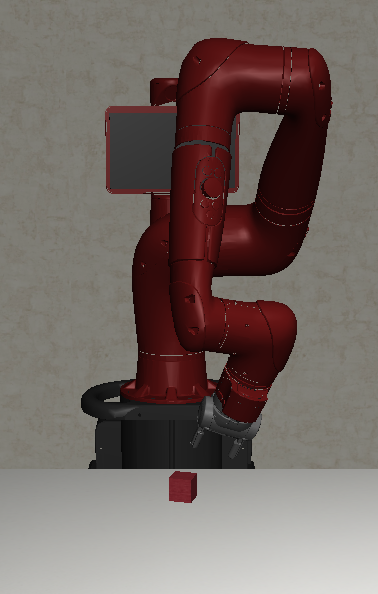
\includegraphics[width=0.2\textwidth]{One_Arm_Env.png}
    \caption{Visual of Robosuite's Lift task.}
    \label{single_arm_env}
\end{figure}

\begin{figure}[h]
    \centering
    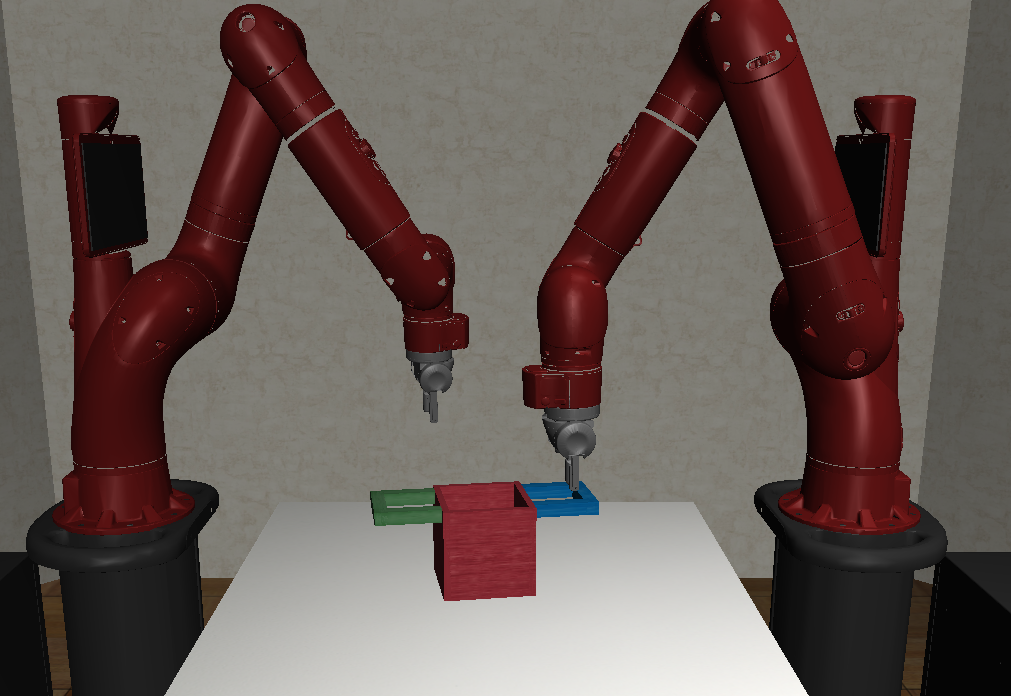
\includegraphics[width=0.4\textwidth]{Two_Arm_Env.png}
    \caption{Visual of Robosuite's Two Arm Lift task.}
    \label{double_arm_env}
\end{figure}

\section{Technical approach}\label{techApp}

\subsection{Network Architectures}
\subsubsection{Estimators}
The partial estimators are the pre-trained networks that are chained together inside of the $f^{composed}$. Each network takes in the robot's state and the action the respective robot plans to execute. The robot's state is the position and orientation of the center of mass of the object. The output of the network is what the expected next state will be. These networks were trained individually from human demonstration data. A simple $\ell_2$ loss metric was used between the predicted next state and actual next state collected by the human demonstrations. All partial estimators had four hidden layers with sixty-four hidden units on each layer.

The full estimator known as $f^{joint}$ takes in the the same information as the partial estimators, but it is trained on reinforcement learning episodes. The input of the state is similar to the partial estimators except it takes in all robot actions at once instead of a single robot's action. The same loss, number of hidden layers, and number of hidden units were used for the full estimator as the partial estimators.

\subsection{Actor-Critic}

The actor network is the policy network that takes in all of the state variables: all robot joint positions, all robot end effector positions, and the position and orientation of the object to be moved. The output of the network are the changes in position and orientation of the robot arms' end effector. The critic network takes in the same data as the actor network, but outputs a scalar value known as the score. We train these networks to maximize the intrinsic and extrinsic reward. The extrinsic reward is the reward assigned by the task. We defined it as the negative of the distance from a robot's end effector to the desired object. The intrinsic reward is the difference between the full estimator and the chained partial estimators. The intrinsic reward favors actions that maximize the difference between individual actions and collective actions. Since the action space is continuous, the rewards are used in a DDPG framework to train the actor and critic networks. Both the actor and critic networks have four layers and have sixty-four units in each hidden layer.

\section{Simulation Results} \label{sec:simu}

For our project proposal, we mentioned that we wanted to add mobility to our robot arms for collision avoidance. We discovered that creating a mobile base was more difficult than we expected. Therefore, all simulations had the robot arms being stationary. Before we came to this decision, we made an environment that had obstacles the robot's were meant to avoid as seen in Figure \ref{newEnvi}. Since the robot's were stationary, we scrapped the environment since the obstacles did not prevent the robot's from achieving their goal.

\begin{figure}[htbp]
    \centering
    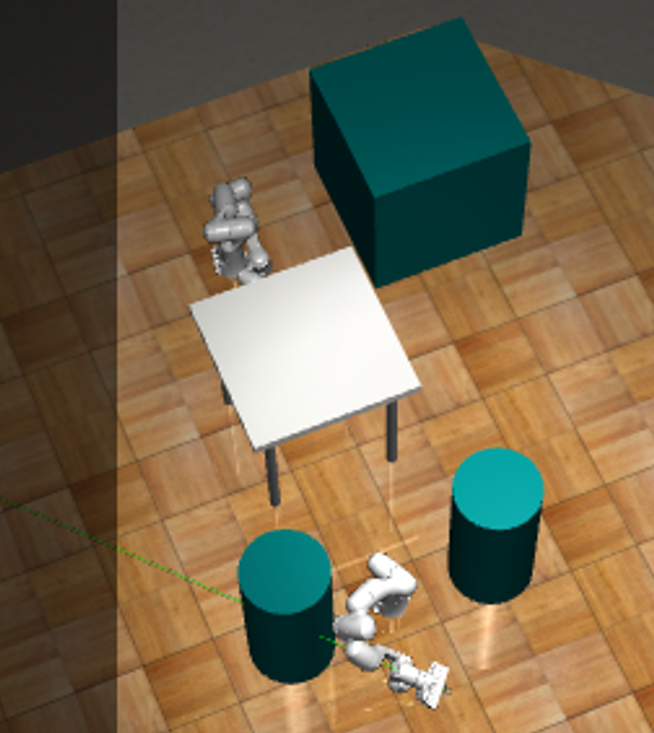
\includegraphics[width=0.4\textwidth]{newEnvi.png}
    \caption{New environment}
    \label{newEnvi}
\end{figure}

While developing our testing methods, we modified the initializer of Robosuite's Lift environment to produce multiple basic 3D shapes of various size and starting locations. However, we could not accurately input the geometries of the 3D shapes into the neural network architectures, so we decided to keep the object's the same shape and size in all experiments.

We experimented with a popular reinforcement learning library called Ray-RLLIB. They have many state-of-the-art implementations of various reinforcement learning neural networks and training methods. Sadly, we could not change the network architecture easily, so we went with other open-source implementations of the RL algorithms we used in this project and will be referenced in the footnotes.

\subsection{DDPG on Fetch Reach}

We used the Deep Deterministic Policy Gradient algorithm to train a robotic arm for the Fetch Reach environment in Gym Open AI \cite{gymopenai}. The DDPG method effectively trains our model in a simple environment\footnote{Source code: \url{https://github.com/vy007vikas/PyTorch-ActorCriticRL}}. Figure \ref{fetch-reach-convergence} shows the total reward of our DDPG algorithm in this environment after a complete epoch. In this case, the environment gives a continuous set of shaped rewards which allows the model to easily find the best motion that maximizes the expected reward. We can see that it is approaching 0 after a small number of episodes. When viewing the learned policy in the testing phase, we saw that it converged to a successful policy\footnote{Video link: https://www.youtube.com/watch?v=f0K8ELWbX18}.

\begin{figure}[h]
    \centering
    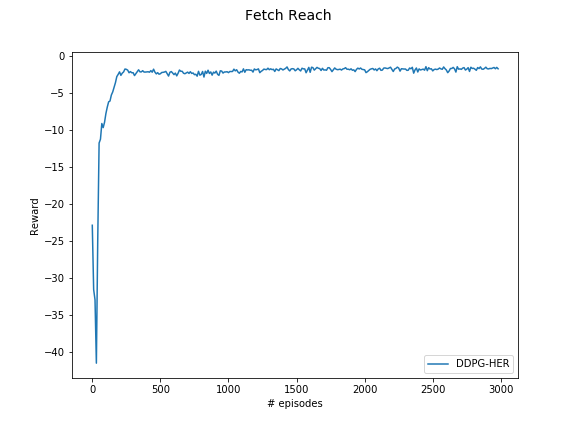
\includegraphics[width=0.48\textwidth]{Fetch Reach.png}
    \caption{Convergence of DDPG in the Fetch Reach environment}
    \label{fetch-reach-convergence}
\end{figure}

\subsection{DDPG+HER on Fetch Pick and Place}

For Fetch pick-and-place environment in Gym Open AI \cite{gymopenai}, the goal for the robot arm is to pick a cube on a table and place it at another location in the 3D space above the table. In this case, the reward is \textit{sparse and binary}, which means that the environment provides a reward of 0 only when the end effector holds the cube at a small distance from the desired location (otherwise the reward is $-1$). It is more difficult to train a model with sparse rewards since at start it is extremely unlikely that the robot will pick-and-place the cube at the desired location. Since the model always receives the same reward ($-1$), there is not feedback to train the model and make it better for the next episodes. That is why the DDPG algorithm is not successful for this environment. For this reason, we combine the DDPG algorithm with HER. As stated in the literature, adding HER improves DDPG methods in a sparse reward environment. We confirmed this with our own results.
The DDPG-HER method effectively trains our model\footnote{Source code: \url{https://github.com/alishbaimran/Robotics-DDPG-HER}.}, and we recorded video of the learned policy\footnote{Video link: \url{https://youtu.be/1MzeGs4A10I}.}. Figure \ref{fetch-pick-place-convergence} shows the success rate of our DDPG-HER algorithm versus the random selection in this environment, we can see that it is progressively reaching 100\% success rate.

\begin{figure}[h]
    \centering
    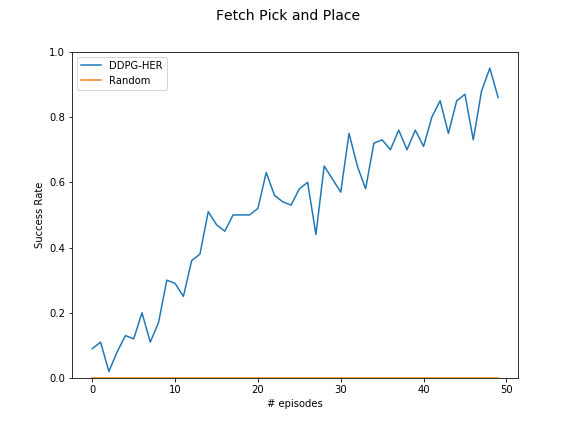
\includegraphics[width=0.48\textwidth]{Fetch Pick and Place.png}
    \caption{Convergence of DDPG-HER in the Fetch pick-and-place environment}
    \label{fetch-pick-place-convergence}
\end{figure}

\subsection{Robosuite Lift}

For the single arm lift task, we were able to find a policy that grasped the cube and moved around in the environment. For our reward function we just reward grasping the object and moving, so the actions the robot arm takes after grasping the object are relatively random\footnote{Video Link: https://youtu.be/r-yUpiwhuF0}. It can be seen that the gripper we selected barely fits the size of the block, so the tolerance in orientation and position for an effective grasp is extremely tight.

\subsection{Robosuite Two Arm Lift}

For the two arm lift task, we were able to find a policy that grasped the handles frequently. However, the lifting aspect of the task was never learned. This is most likely due to the reward shaping we used over weighting the grasping handle action more than the object going to its goal position. Interestingly, the policy to put the grippers around the handles converged pretty quickly after only a few dozen epochs. This was most likely due to the handles width being much skinnier than the open position of the grippers. In the block lifting task for the single arm, the agent had little affordance for orientation and position of the gripper in order to achieve a strong grasp on the object.

\section{Conclusion} \label{sec:ccl}

In this paper, we presented a synergetic algorithm aiming at using multiple robots for manipulation tasks. Our key results show that the deep deterministic policy gradient algorithm is not efficient for complex environments with sparse rewards, which are the most realistic types of reward. To solve the issue, hindsight experience replay is a strong tool that can be wrapped around DDPG to make the model learn in such complex environments. In this case, DDPG+HER efficiently achieves a high success rate in picking up and placing objects.

In future research, the work can be extended to synchronize the two robotics arms and make them collaborate to lift a unique object. It could then be further extended to more than two robots for objects that are difficult to grasp. Additionally, incorporating mobile robots will add other challenges due to the higher number of degrees of freedom but it will open new possibilities for multi-agent mobile manipulation. Specifically, such systems are relevant in industrial robotics, for packages delivery, etc.

\bibliographystyle{IEEEtran}
\bibliography{ref}

\end{document}


